\documentclass{tietreport}

\usepackage{graphicx}
\usepackage{amssymb}

\usepackage[
  date=year,
  style=alphabetic,
  backend=biber,
  sorting=nty,
  maxnames=5,
  minnames=3,
  maxalphanames=4,
  minalphanames=3,
  backref=true,
  doi=false,
  isbn=false,
  url=false,
  eprint=false
]{biblatex}

\addbibresource{references.bib}

\usepackage{xcolor}

\setlength{\headheight}{14.5pt}
\addtolength{\topmargin}{-2.5pt}


\TitlePageHeader{%
  UCS 503P --- Software Engineering Project%
}

\ProjectTitle{%
  UniVerse: A Skill Swap Community Platform%
}

\ProjectSubTitle{%
  Peer-to-Peer Teaching Platform with Real-Time Chat and Credit-Based Incentives%
}

\author{%
  \texttt{1024030215} Sehajneet Kaur \\
  \texttt{1024030711} Raynee Jindal \\
  \texttt{1024030247} Sahejbir Singh \\
  \texttt{1024030649} Shaurya Ranjan%
}

\TitlePageSubText{%
  Group: \texttt{3C52} BE Third Year, COE%
}

\AdvisorName{%
  Paramveer Kaur Ma'am%
}

\TitlePageFooterText{{%
    \large Project Report Prototype Stage \\[0.2cm]
    \bfseries Computer Science and Engineering
    Department%
  } \\[0.15cm]
  Thapar Institute of Engineering and Technology,
  Patiala%
}

\let\cleardoublepage\clearpage
\begin{document}

\maketitle

\tableofcontents


\chapter{Introduction}

\section{Background and Context}

UniVerse is a web-based peer-to-peer skill exchange platform designed exclusively for the Thapar Institute of Engineering and Technology (TIET) community. Students possess diverse skills but lack a structured, incentivized way to teach and learn from one another. The motivation behind UniVerse stems from three observations:

\begin{enumerate}
  \item \textbf{Unutilized Peer Expertise:} Students often struggle to find classmates with specific skills.
  \item \textbf{Resource Inefficiency:} Books and lab equipment are borrowed informally or through inefficient channels.
  \item \textbf{Community Isolation:} The campus lacks a unified channel for lost-and-found, discussions, and resource exchange.
\end{enumerate}

\subsection{Problem Statement}

Students at TIET require a platform to:

\begin{itemize}
  \item Discover and request peer-taught sessions, and offer their own skills to peers.
  \item Coordinate learning through real-time chat.
  \item Borrow, lend, and report lost items across the community.
\end{itemize}

\section{Project Objectives}

\begin{enumerate}
  \item \textbf{Skill swap subsystem:} Enable students to offer and request peer-taught sessions with real-time negotiation via chat.
  \item \textbf{Credit-based incentive system:} Reward teaching (+10 credits per session) and deduct for learning (-5 credits per session) with atomic correctness.
  \item \textbf{Community and admin features:} Support borrow/lend posts, lost-and-found reports, discussions, and moderation tools.
  \item \textbf{Security:} Restrict access to @thapar.edu accounts and enforce role-based authorization.
\end{enumerate}

\section{Project Scope}

\begin{itemize}
  \item \textbf{User Base:} TIET students with valid @thapar.edu Google accounts only.
  \item \textbf{Core Features:} Skill Swap, Utility Channels (General, Borrow/Lend, Lost \& Found), real-time chat, notifications, and admin management.
\end{itemize}


\chapter{Methodology and Design}

\item \textbf{The project followed an iterative, feature-by-feature development approach.}

\section{System Architecture}

UniVerse is a three-tier web application:

\begin{enumerate}
  \item \textbf{Frontend:} React 18 + Vite, communicating with the backend via REST API and WebSocket.
  \item \textbf{Backend:} Node.js + Express 5, implementing business logic, authentication, authorization, and real-time messaging.
  \item \textbf{Data Layer:} MongoDB Atlas, storing user profiles, skills, sessions, posts, messages, and transactions.
\end{enumerate}

\subsection{High-Level Design}

\subsubsection{Authentication Flow}

\begin{itemize}
  \item Google OAuth 2.0 is the sole authentication mechanism, restricted to the @thapar.edu domain.
  \item A short-lived JWT access token and a refresh token are issued as HTTP-only cookies.
\end{itemize}

\subsubsection{Credit System}

\begin{itemize}
  \item New users start with 50 credits; a completed session gives the mentor +10 and charges the learner -5.
  \item Credit updates use MongoDB atomic operations, and session completion is idempotent.
  \item Admins can deduct credits with a mandatory reason (e.g., no-show penalty).
\end{itemize}

\subsubsection{Real-Time Messaging}

\begin{itemize}
  \item Socket.IO enables one-to-one chat between session participants, authenticated with JWT.
  \item All messages are persisted to MongoDB so history survives disconnections.
\end{itemize}

\subsubsection{Community Channels}

\begin{itemize}
  \item Three fixed channels: General, Borrow/Lend, and Lost \& Found.
  \item Posts in Borrow/Lend and Lost \& Found can be closed, after which no interactions are allowed.
  \item General supports upvotes/downvotes, nested comments, saving, and reporting.
\end{itemize}


\subsection{Activity Diagram}

Figure~\ref{fig:activity} shows the skill swap workflow, from listing a skill to rating the session.

\begin{figure}[htbp]
  \centering
  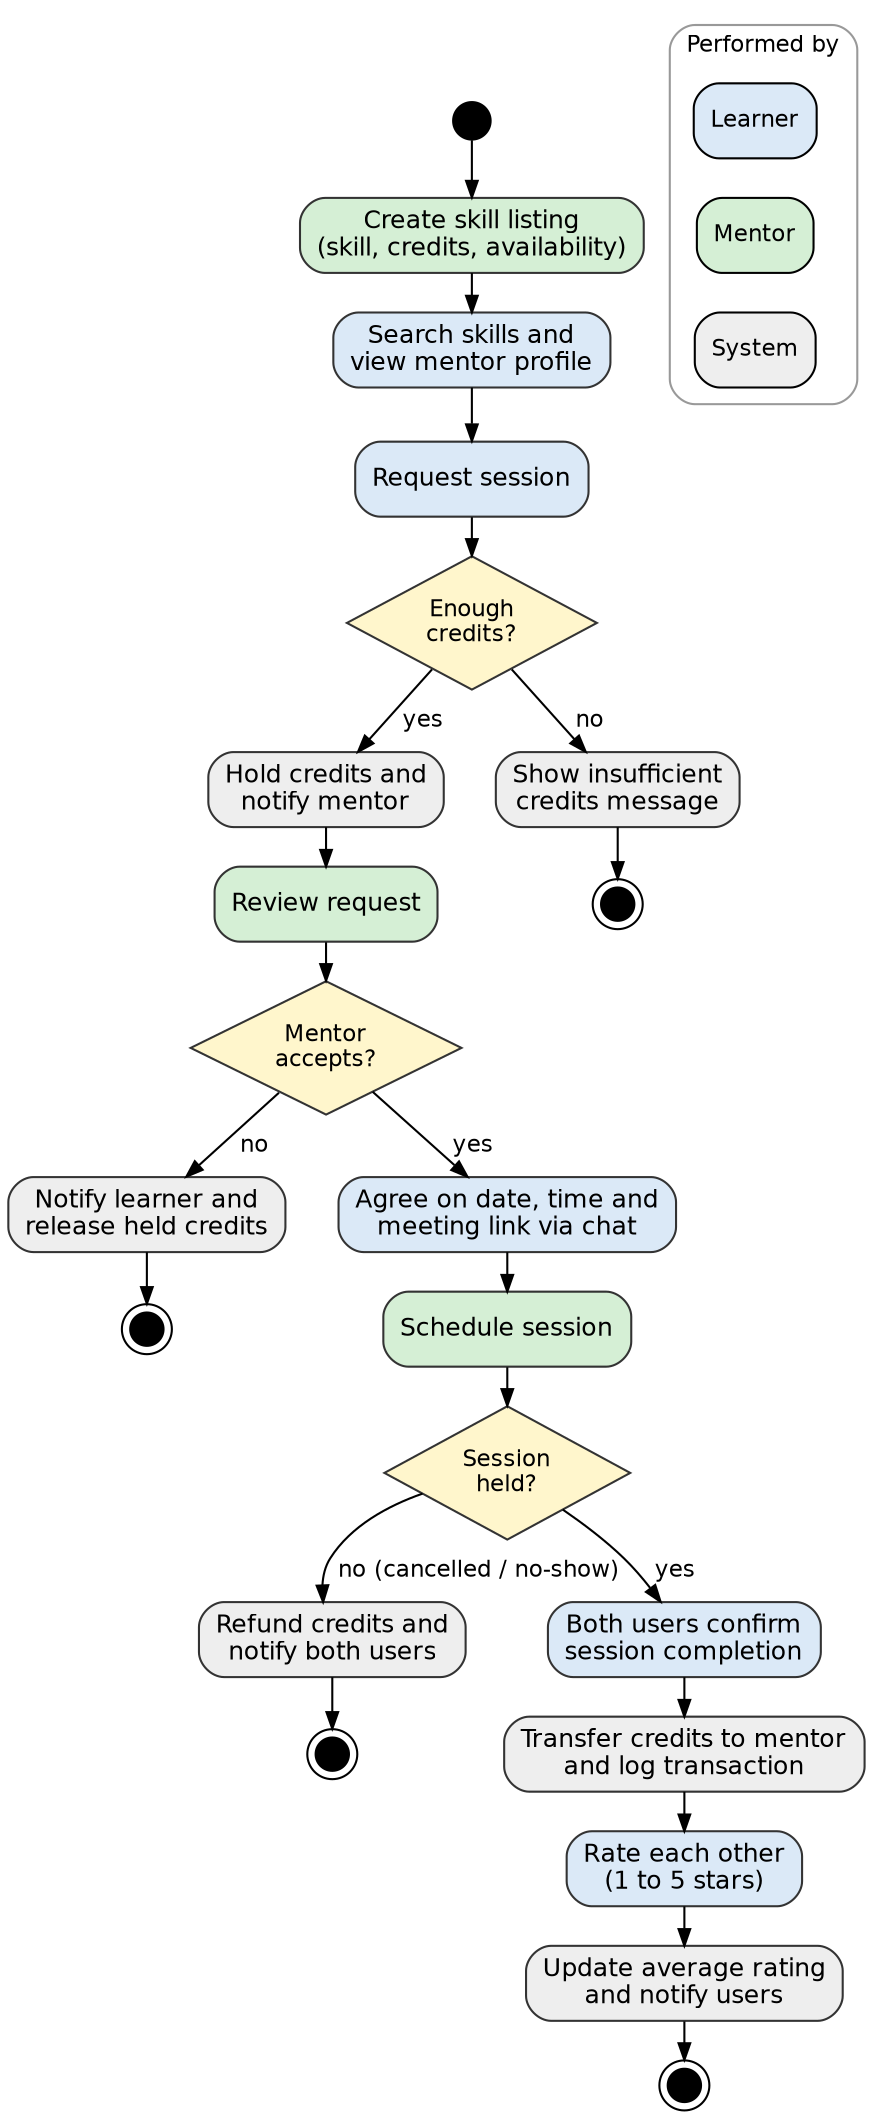
\includegraphics[width=\linewidth,height=0.85\textheight,keepaspectratio]{activity_diagram.png}
  \caption{Skill Swap Activity Diagram}
  \label{fig:activity}
\end{figure}

\subsection{Class Diagram}

Figure~\ref{fig:classdiagram} shows the UML class diagram of the main entities, their key attributes, public methods, and relationships. Enumeration-typed fields (e.g., \texttt{SessionStatus}, \texttt{ChannelType}) are shown by their type name.

\begin{figure}[htbp]
  \centering
  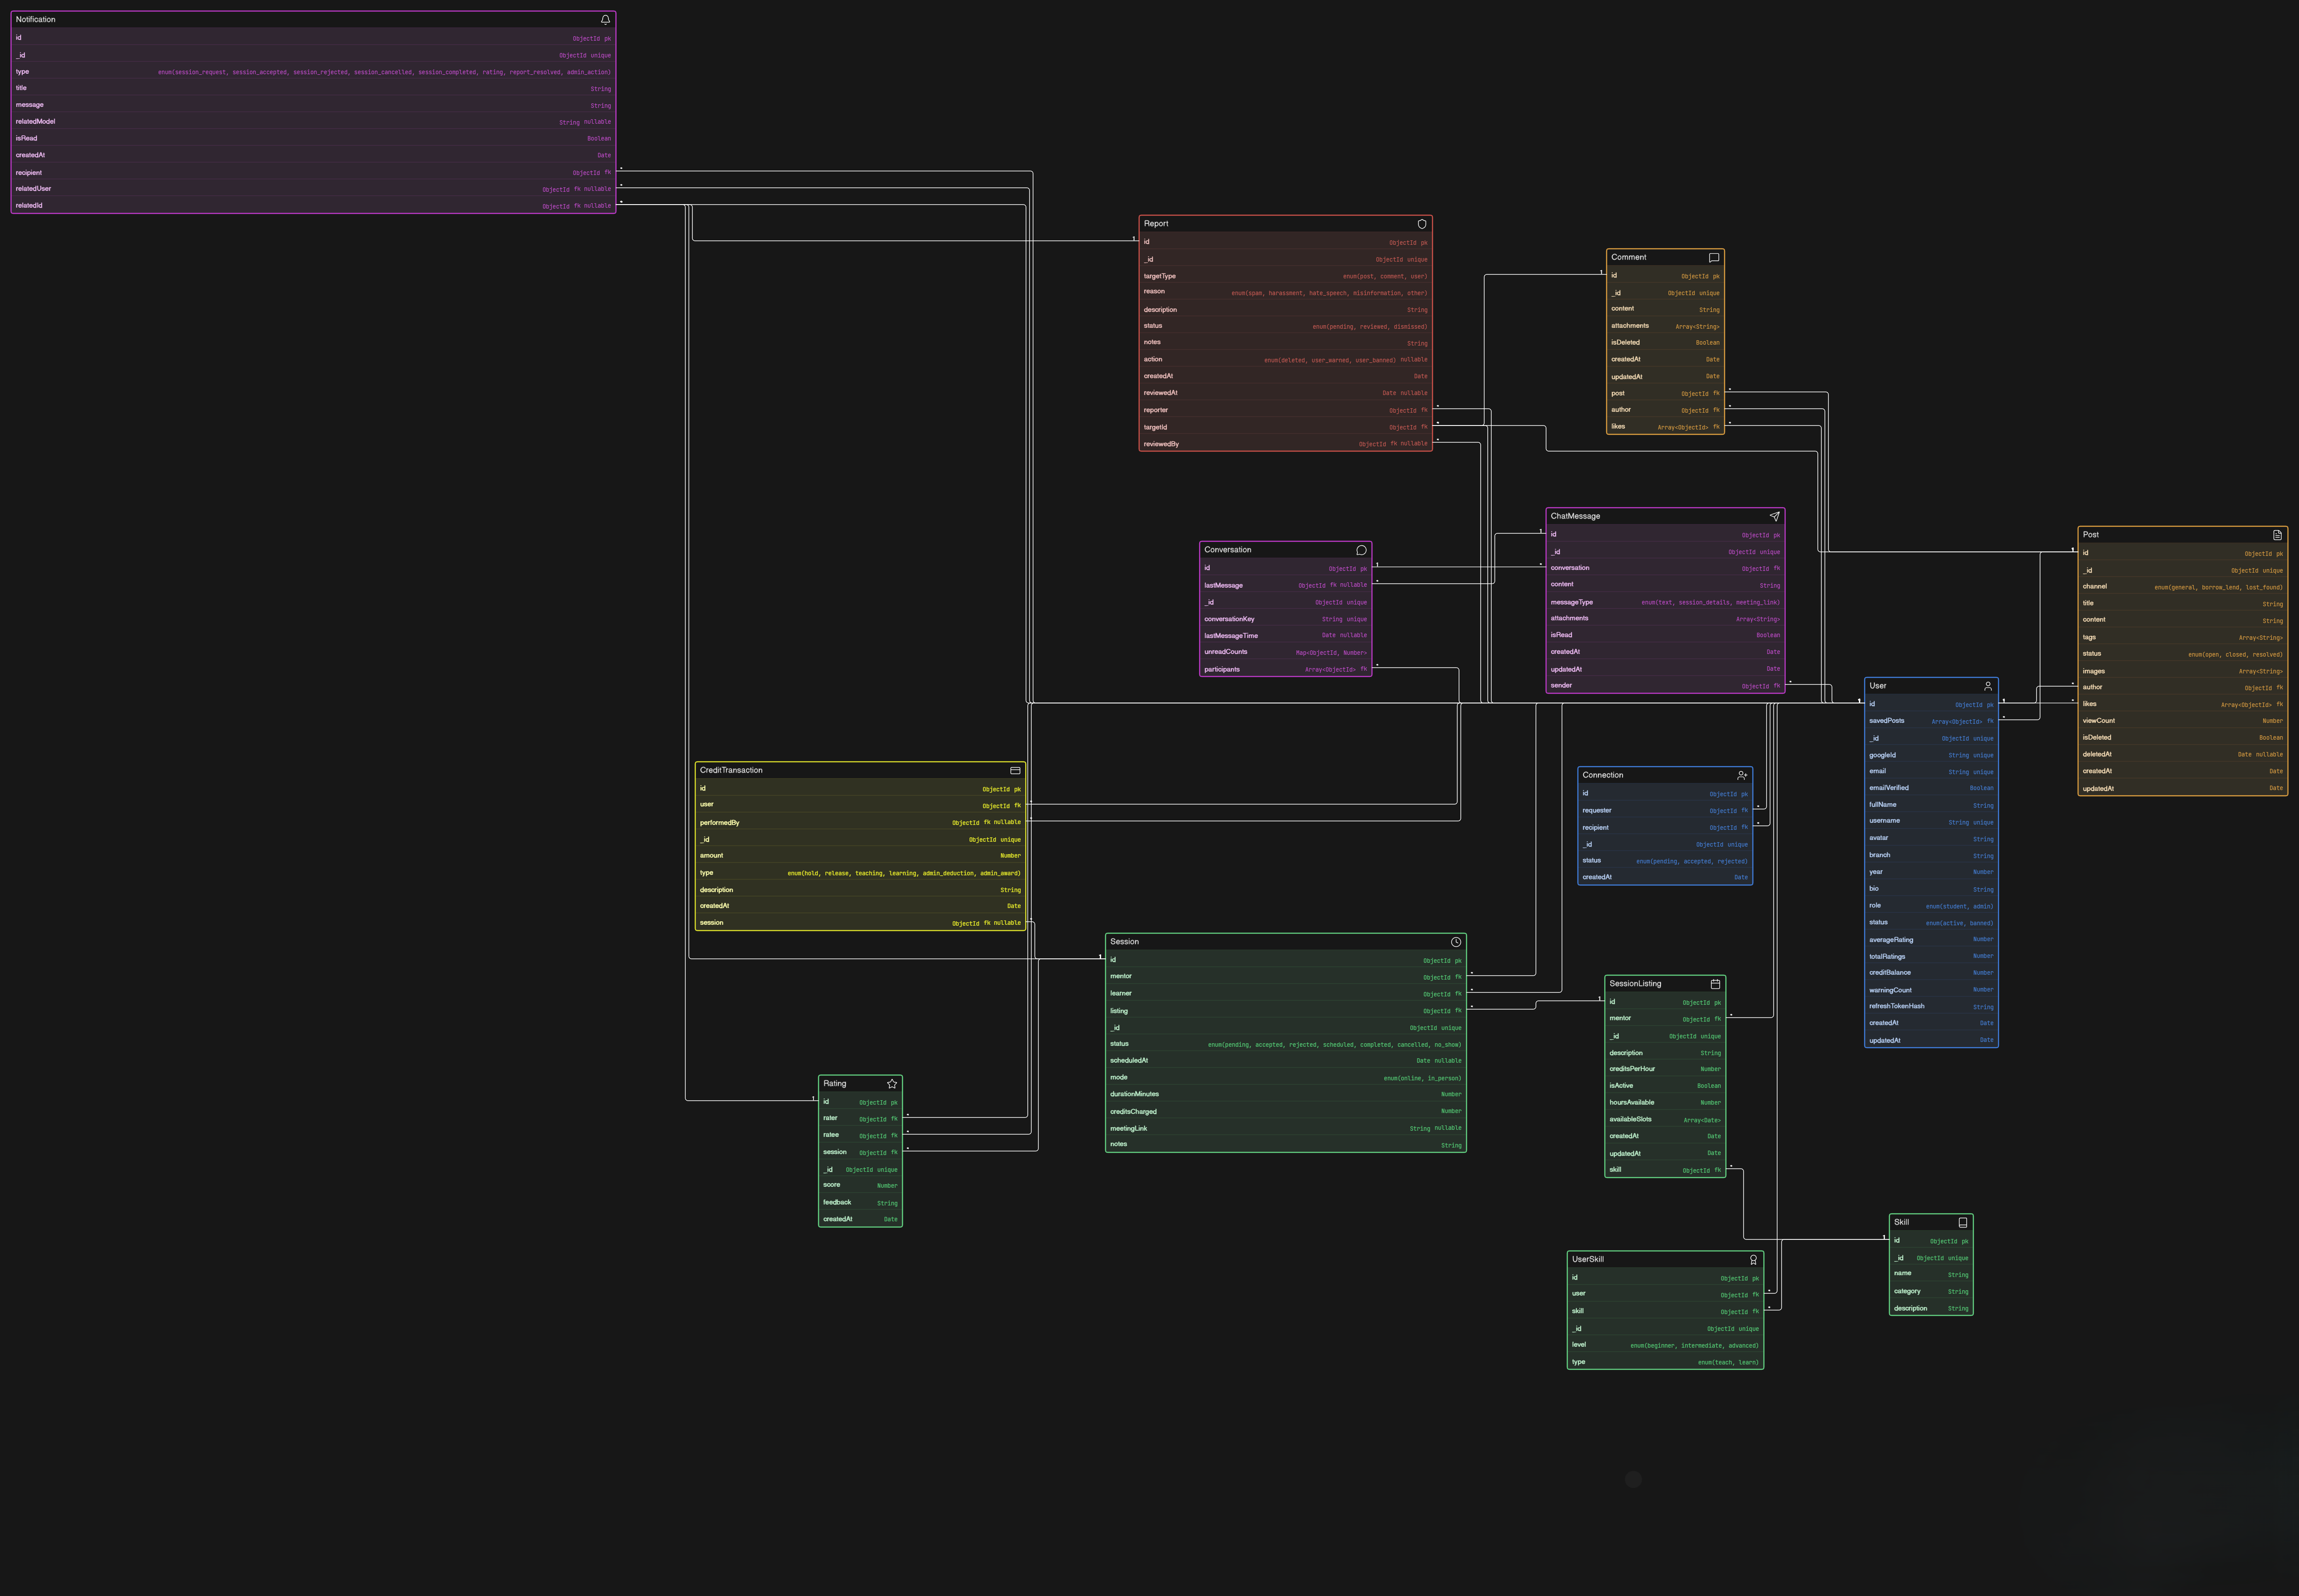
\includegraphics[width=\linewidth,height=0.85\textheight,keepaspectratio]{class_diagram.png}
  \caption{UniVerse UML Class Diagram}
  \label{fig:classdiagram}
\end{figure}

\subsection{Technical Stack}

\begin{itemize}
  \item \textbf{Frontend:} React 18, Vite, React Query, Axios, Socket.IO Client.
  \item \textbf{Backend:} Node.js, Express 5, Mongoose, Socket.IO.
  \item \textbf{Database and Services:} MongoDB Atlas, Google OAuth 2.0, Cloudinary (image storage).
\end{itemize}

\section{Implementation Details}

\subsection{Backend Modules}

\begin{itemize}
  \item \textbf{Authentication:} Google OAuth callback with domain validation, JWT generation, and profile/avatar updates.
  \item \textbf{Sessions and Credits:} Session lifecycle (pending $\rightarrow$ accepted $\rightarrow$ scheduled $\rightarrow$ completed) with atomic credit updates and transaction logging.
  \item \textbf{Posts and Comments:} Post creation with images, nested comments, and closed-post enforcement.
  \item \textbf{Admin:} User suspension/banning, content removal, report review, and credit deduction.
\end{itemize}

\subsection{Database Schema Highlights}

\begin{itemize}
  \item \textbf{User:} profile details, credits (default 50, minimum 0), role, status, and skills to teach/learn.
  \item \textbf{Session:} mentor, learner, skill, status, mode, date, and meeting link.
  \item \textbf{CreditTransaction:} user, amount, type, and session reference for an audit trail.
\end{itemize}

\subsection{Security Measures}

\begin{enumerate}
  \item \textbf{Google OAuth:} Only @thapar.edu accounts can sign in; tokens are stored in HTTP-only cookies.
  \item \textbf{Admin Authorization:} Role-based access control ensures only admins can access admin endpoints.
  \item \textbf{Rate Limiting:} Auth and general API endpoints are rate-limited to mitigate brute-force attacks.
\end{enumerate}

\section{Frontend Architecture}

\begin{itemize}
  \item \textbf{State Management:} Context API with \texttt{useReducer} for authentication, and React Query for server state.
  \item \textbf{Real-Time Chat:} Socket.IO client connection authenticated with JWT.
  \item \textbf{Routing:} React Router v6 with protected routes for authenticated pages.
\end{itemize}


\chapter{Results and Evaluation}

\section{Development Milestones}

\begin{table}[h]
\centering
\begin{tabular}{|l|l|}
  \hline
  \textbf{Milestone} & \textbf{Status} \\
  \hline
  Backend API & Completed \\
  \hline
  MongoDB Schema & Completed \\
  \hline
  Authentication & Completed \\
  \hline
  Credit System & Completed \\
  \hline
  Frontend Components & Completed \\
  \hline
  Real-Time Chat (Socket.IO) & Completed \\
  \hline
  Admin Features & Completed \\
  \hline
\end{tabular}
\caption{Development Milestones and Status}
\label{tab:milestones}
\end{table}

\section{Testing Strategy}

\subsection{Unit Testing}

\begin{itemize}
  \item Credit calculation logic (teach +10, learn -5, floor at 0).
  \item Session status transitions and authorization checks.
\end{itemize}

\subsection{Integration Testing}

\begin{itemize}
  \item End-to-end authentication flow (Google OAuth, token refresh, logout).
  \item Session completion with credit transfer.
  \item Real-time chat message persistence and retrieval.
\end{itemize}

\subsection{Security Testing}

\begin{itemize}
  \item Non-Thapar accounts are rejected at the OAuth callback.
  \item Non-admin users cannot access admin endpoints.
  \item Credits cannot go negative.
\end{itemize}

\section{Challenges Encountered and Resolution}

\subsection{Challenge 1: Cloudinary Image Cleanup}

\textbf{Problem:} When users delete posts or upload new avatars, orphaned images remain in Cloudinary, consuming storage quota.

\textbf{Solution:} Implemented cleanup routines in the post deletion and avatar update controllers that delete the old image through Cloudinary's API.

\textbf{Result:} No orphaned images remained after testing.

\subsection{Challenge 2: Real-Time Chat with Persistence}

\textbf{Problem:} Socket.IO messages are ephemeral; if a user disconnects, message history is lost.

\textbf{Solution:} All messages are persisted to MongoDB with a compound index on (\texttt{conversationId, createdAt}). On reconnection, the frontend fetches recent history from the API.

\textbf{Result:} Chat history survives page reloads and network disconnections.

\subsection{Challenge 3: Closed Post Enforcement}

\textbf{Problem:} Frontend-only enforcement can be bypassed by direct API calls.

\textbf{Solution:} Enforcement was moved to the backend controllers, which return a 409 Conflict response when a user interacts with a closed post.

\textbf{Result:} No interactions are possible on closed posts, even via direct API calls.

\chapter{Conclusion}

\section{Summary of Work}

UniVerse realizes a full-stack peer-to-peer skill exchange platform tailored for the TIET community. The team delivered:

\begin{enumerate}
  \item A backend API supporting authentication, skill discovery, session management, credit transactions, community channels, and admin tooling.
  \item A credit-based economy that incentivizes teaching while keeping learning accessible.
  \item Real-time chat with persistent message history for coordinating sessions.
\end{enumerate}

\section{Key Findings}

\begin{itemize}
  \item \textbf{Atomic Operations are Critical:} The credit system's correctness depends on atomic database operations.
  \item \textbf{Backend-First Security:} Business rules must be enforced on the backend; frontend validation is only for user experience.
  \item \textbf{Persistence for Real-Time Features:} Pairing Socket.IO with MongoDB lets chat history survive disconnections.
\end{itemize}

\section{Future Work and Recommendations}

\begin{enumerate}
  \item \textbf{Deployment:} The platform is not yet deployed. Host the frontend, backend, and database on production infrastructure so it is available to the TIET community.
  \item \textbf{User Search:} Add user search based on rating, which is not implemented yet.
  \item \textbf{Skill Proficiency Levels:} Extend the Skill model with proficiency levels (Beginner, Intermediate, Advanced) for more granular matching.
  \item \textbf{Recommendation Engine:} Build a machine learning model to recommend skills to learn based on user history and peer trends.
\end{enumerate}

\section{Learning Outcomes}

\begin{itemize}
  \item \textbf{Distributed Systems:} Race conditions, atomicity, and idempotency.
  \item \textbf{Security:} OAuth flows, JWT token management, and role-based authorization.
  \item \textbf{Real-Time Communication:} WebSocket fundamentals and persistence strategies.
\end{itemize}

\section{Final Remarks}

UniVerse shows that a peer-to-peer community platform can be built with modern technologies. The combination of a credit system, real-time communication, and community channels gives students a reason to participate and invest in their peers' growth. With deployment and the planned enhancements, it can become a useful platform for informal learning at TIET.

\nocite{*}
\printbibliography[heading=bibintoc]

\end{document}